\documentclass[letterpaper,10pt,titlepage]{article}

\usepackage{amsmath}                                         
\usepackage{amsthm}

\usepackage{alltt}                                           
\usepackage{float}
\usepackage{color}

\usepackage{balance}
\usepackage[TABBOTCAP, tight]{subfigure}
\usepackage{enumitem}

\usepackage{pstricks, pst-node}
\usepackage{geometry}
\usepackage{graphicx}
\geometry{textheight=10in, textwidth=7.5in}
%random comment

\newcommand{\cred}[1]{{\color{red}#1}}
\newcommand{\cblue}[1]{{\color{blue}#1}}

\usepackage{hyperref}

\def\name{David Merrick}


%% The following metadata will show up in the PDF properties
\hypersetup{
  colorlinks = true,
  urlcolor = black,
  pdfauthor = {\name},
  pdfkeywords = {cs311 ``operating systems'' pipes signals},
  pdftitle = {CS 311 Project 4: Thread primes},
  pdfsubject = {CS 311 Project 4},
  pdfpagemode = UseNone
}

\parindent = 0.0 in
\parskip = 0.2 in

\begin{document}
David Merrick

CS 311

1 March, 2013

\begin{center}
{\LARGE Writeup for Assignment 4}
\end{center}

\begin{enumerate}
\item \emph{A design for your system, as well as places your implementation deviated from this design.}
\begin{figure}[htp]
  \begin{center}
  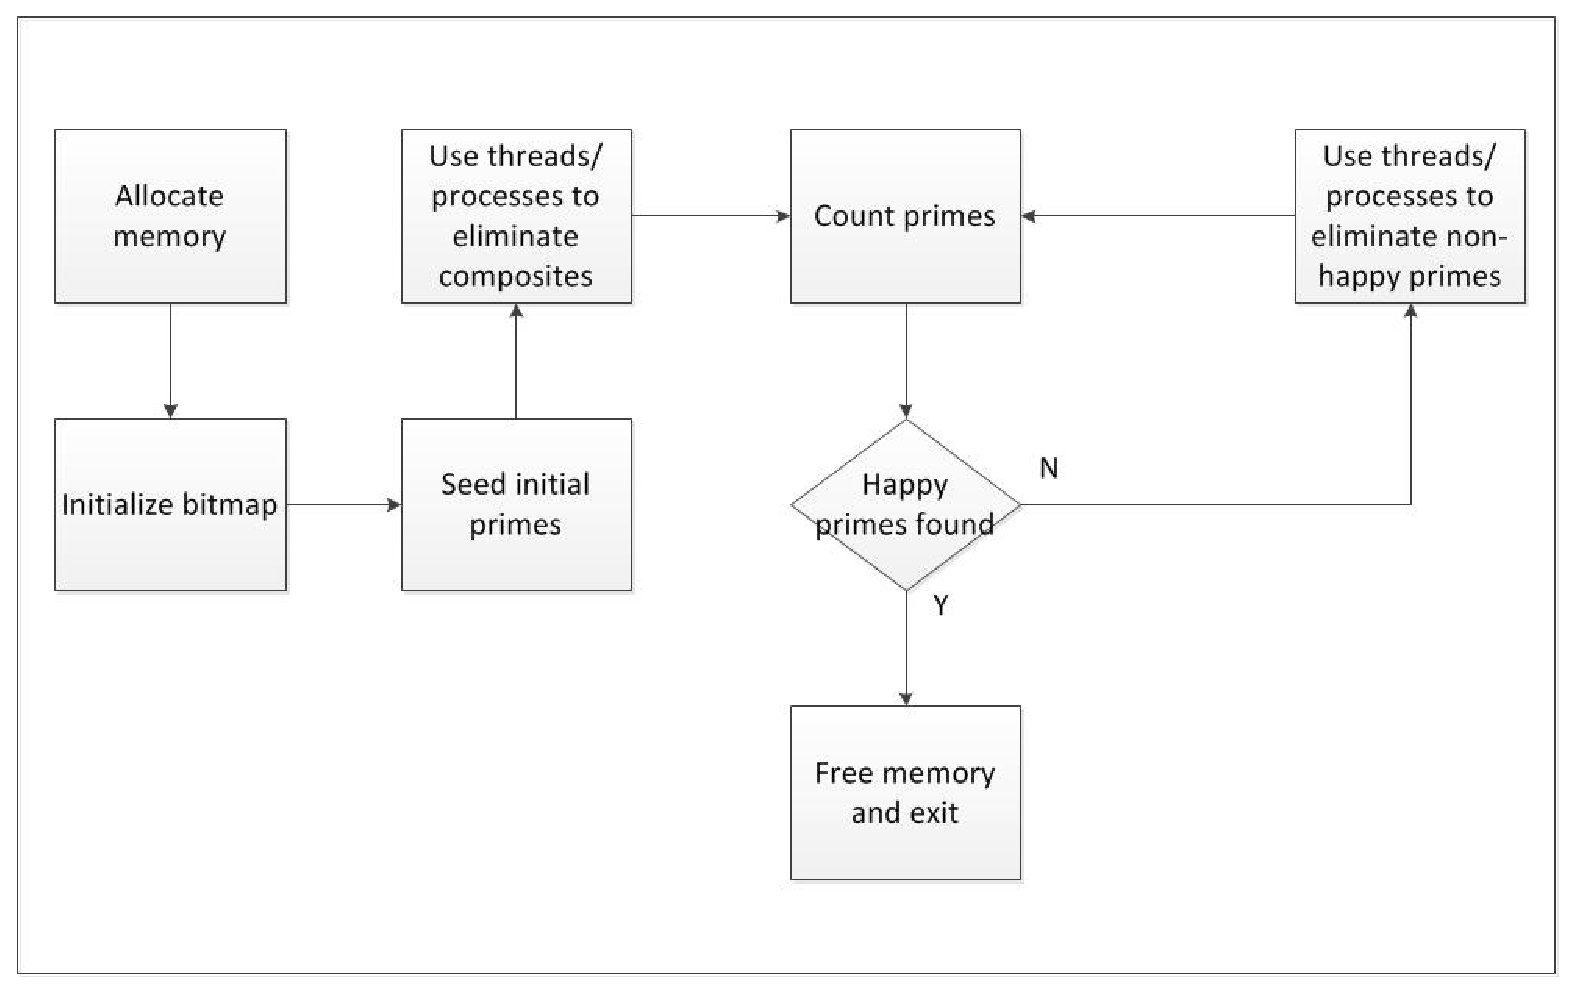
\includegraphics[width=8in]{design_flowchart}
  \end{center}
  \caption{Modular flowchart design for my programs.}
\end{figure}

My design was initially very black-box and modular, as I was not sure which algorithm I would use for finding the primes. All of the algorithms I was aware of, however, seeded a list of primes or candidate primes and then eliminated composites. I knew that I would first need to mount shared memory or malloc, initialize the bitmap, seed the initial primes, then spawn threads or processes to eliminate composites, count the primes, then use threads or processes to find the happy primes, count the happy primes, and then free the memory. I made each of these into a module that called other functions within it. Designing it with this level of abstraction gave me the ability to optimize each module without affecting the performance of the others, and test which optimization made the program the fastest. It also gave me the flexibility of testing different prime algorithms without having to rewrite significant portions of my code.

\item \emph{Work Log:}

2013-03-01 12:05:53 -0800, Added plots file for writeup

2013-03-01 11:04:08 -0800, Fixed syntax errors in tprimes, ran python script to run program over and over to generate data for plots.

2013-03-01 10:45:57 -0800, Made updates to both programs. Added -d option to suppress output for testing. Pprimes signal handling is also working.

2013-02-28 20:08:33 -0800, There is a bug in my signal handler. Will ask him about it tomorrow.

2013-02-28 19:02:57 -0800, Wrote Python script to run tests on programs and output of those tests

2013-02-28 17:44:56 -0800, Made a version of tprimes that outputs a csv of num\_threads, max\_prime, and prime calculation time for purposes of writeup.

2013-02-28 17:34:04 -0800, Added command line arguments

2013-02-28 17:19:06 -0800, Added code to record timings of finding the primes

2013-02-27 22:55:58 -0800, Changed searching convergence array to binary search algorithm. Not sure if the math adds more overhead, especially in such a small array. Didn't seem to boost performance like I was hoping it would

2013-02-27 18:11:36 -0800, Got primes working with processes. Just need to fix signal handling

2013-02-27 17:24:34 -0800, Created primes file using processes

2013-02-27 17:10:12 -0800, Optimized code for counting primes and finding next prime. Shaved about a minute off time to compute and count happys.

2013-02-27 14:20:26 -0800, Fixed bottleneck. It was in the nextprime function where I was using unsigned int for i instead of long.

2013-02-27 13:28:50 -0800, Finds happy primes successfully but is really slow. Pushing this so I can debug.

2013-02-26 21:01:54 -0800, Made some updates, compiles but there are some bugs in the finding happy primes. Pretty sure there is an infinite loop somewhere.

2013-02-26 18:16:02 -0800, Added basic Happy Prime functionality. Have not tested yet.

2013-02-26 15:18:55 -0800, Got it finding the correct number of primes.

2013-02-26 14:39:28 -0800, Added signal handler that deletes shared memory

2013-02-26 13:56:55 -0800, Got a thread argument passed as a struct, but might need a mutex for this. To eliminate overhead, will rewrite to just pass unsigned int to thread. Pushing this to GitHub because I might revisit it later during optimization.

2013-02-25 13:45:04 -0800, Successfully added parallelism to initializing candidate primes. They're 1 off right now, but I do not think the bug is in the primes algorithm. To do: Add a semaphore to protect array during this initialization process.

2013-02-25 13:18:42 -0800, Sieve of Atkin is working successfully. Can find all primes from 1 to 4 billion in about 5 min serially. Now to parallelize it.

2013-02-25 12:14:11 -0800, Got Sieve of Atkin algorithm working

2013-02-24 17:09:07 -0800, Impemented bitmap for primes plus functions for initializing and modifying it. Find\_primes isn't working now though.

2013-02-23 17:54:18 -0800, Implemented mutex to guard numprimes variable. But am getting 1874 for the number of primes from 1 to 10,000 when I should be getting 1229.

2013-02-23 17:38:11 -0800, Added helpful example files for reference.

2013-02-23 17:09:57 -0800, Implemented threads. Just 2 of them. Threading is working but am getting incorrect number of primes.

2013-02-23 15:51:11 -0800, In the makefile, if openmp is specified, this segfaults. If not, works fine. But gcc doesn't work in any case.

2013-02-23 14:59:34 -0800, Added example code from class on mounting shared memory objects

\item \emph{Timings:}
\begin{figure}[H] %H places the figure HERE. Requires float package.
  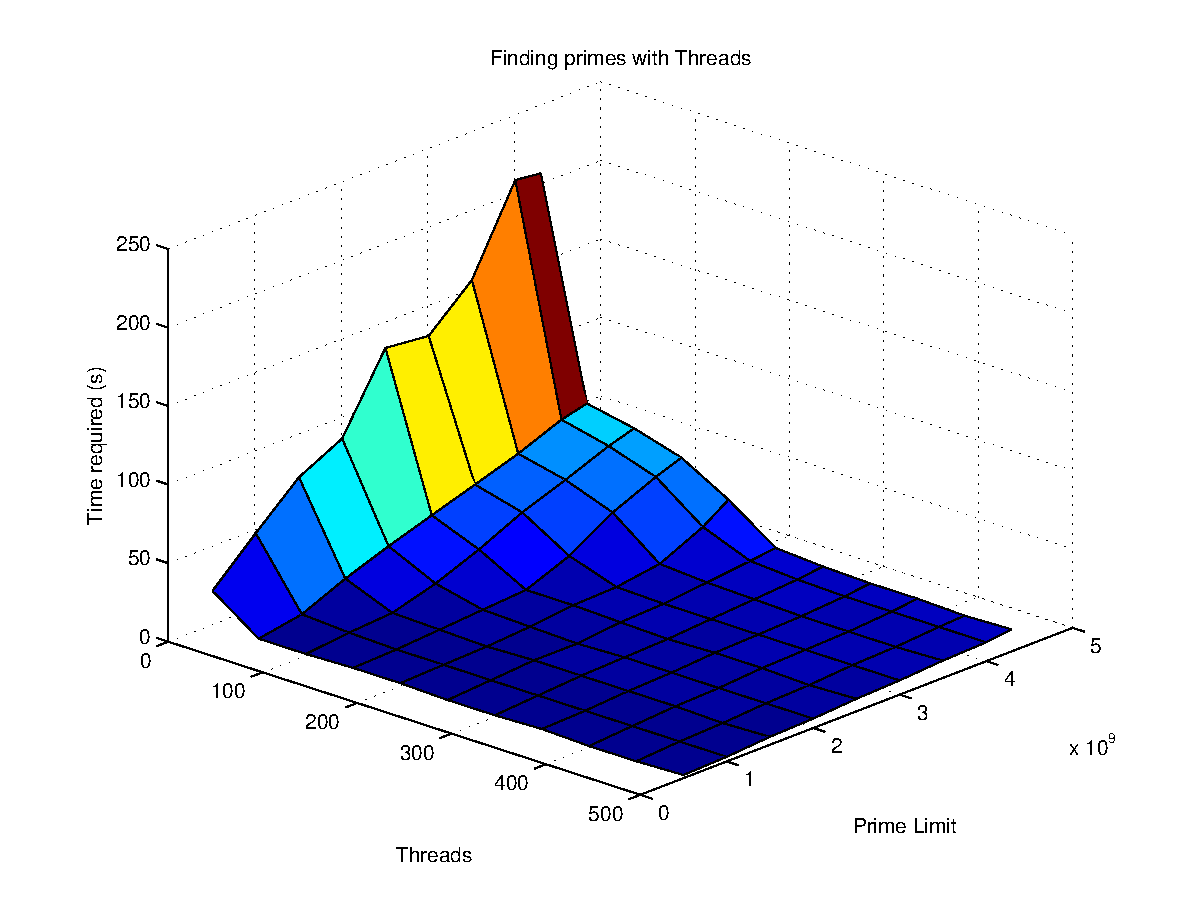
\includegraphics[width=4in]{tplot}
  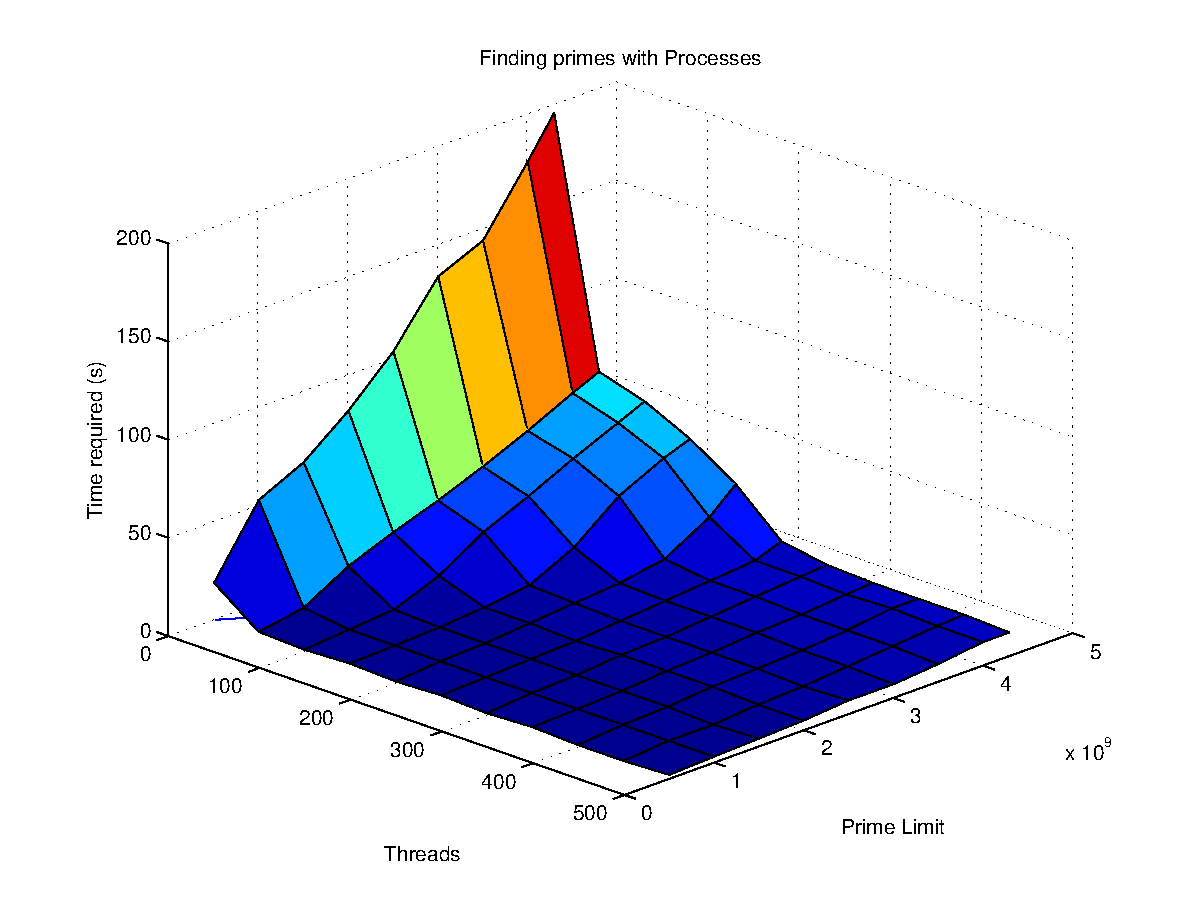
\includegraphics[width=4in]{pplot}
\end{figure}

The threads and processes performed with very similar timings on varied numbers of primes and varied numbers of processes. With 500 threads, my program found the primes up to 4294967295 in approximately 14 seconds. With 500 processes on this same limit, it took approximately 12 seconds. This variation could easily be explained by a difference in a system state, such as another user running their program concurrently.

\item \emph{Challenges:}
The biggest challenge was debugging. I was not able to figure out how to step into the threads with GDB, so my threads were like a black box after they started. I got around this by using print statements within the threads to ensure they were calculating the correct ranges and that there were no infinite loops. I tested my program\'s performance on relatively small numbers of primes. Once I got this working, I increased the number of threads to make sure it still worked correctly. Then I steadily increased the number of primes. Another challenge was using the bitmap. Initially, I was very confused about how to set it up and why we were using one. Once I realized how efficient it was, and how easy it was to set and unset bits, I created the functions "set\_prime", "set\_not\_prime", and "is\_prime" to abstract setting, unsetting, and checking bits in the bitmap, respectively.

\end{enumerate}

%input the pygmentized output of mt19937ar.c, using a (hopefully) unique name
%this file only exists at compile time. Feel free to change that.
%\input{__mt.h.tex}
\end{document}
